\documentclass[a4paper]{article}

\usepackage[T3]{fontenc}
\usepackage[utf8]{inputenc}
\usepackage[russian]{babel}

\usepackage{fullpage} % Package to use full page
\usepackage{parskip} % Package to tweak paragraph skipping

\usepackage{amsmath, amssymb}
\usepackage{graphicx}
\usepackage[colorinlistoftodos]{todonotes}

\usepackage{mhchem}

\title{Отчет.}

\date{\today}

\begin{document}
\maketitle

\begin{abstract}
Abstract.
\end{abstract}

\section*{Синтез 2-бензолиденциклопентанона.}
\begin{center}
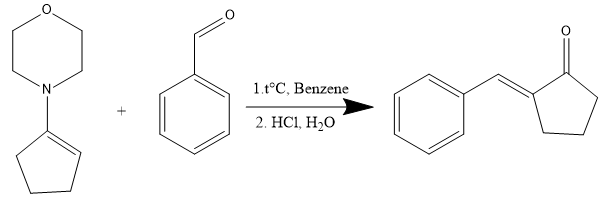
\includegraphics[scale=0.5]{pictures/1.png}
\end{center}
11.45г (74.84 ммоль) N-циклопентанилморфолина, 6.61г (62.36 ммоль) свежеперегнанного бензальдегида и 60 мл бензола помещают в круглодонную колбу и нагревают с насадкой Дина-Старка в течение 20 часов. За ходом реакции следят при помощи ТСХ (элюент -- петролейный эфир : этилацетат, 4 : 1).
Затем раствор охлаждают до комнатной температуры и при перемешивании добавляют 43.5 мл 6М $\ce{HCl}$. После перемешивания в течение 2 часов органический слой отделяют и промывают водой до нейтрального pH, оставляют сушиться над $\ce{Na2SO4}$ на ночь. Затем смесь фильтруют и отгоняют бензол на роторном растворителе. Остаток охлаждают и кристаллизуют. Очистку производят перекристаллизацией из смеси этанол - циклогексан.

\section*{Синтез 2-бензолиден-5-(4-метоксибензолиден)циклопентанона.}
172 мг  моноенона, 136 мг анисового альдегида, 230 мкл 2N $\ce{NaOH}$ и 1.5мл $\ce{EtOH}$ помещают в круглодонную колбу и перемешивают в течение часа. Реакция протекает при комнатной температуре, за ходом реакции следят при помощи ТСХ. Реакция сопровождается выпадением грязно-желтого осадка диенона. После окончания реакции реакционную смесь переносят на фильтр со стеклянным фильтрующим дном, осадок промывают небольшими количествами воды, сушат в пистолете Фишера. 
Выход: 40.69$\%$ (от теории).

\section*{Синтез 2-бензолиден-5-(пиридин-3-илметилен)циклопентанона.}
172 мг моноенона, 107 мг 3-пиридинкарбальдегида, 330 мкл 2N $\ce{NaOH}$ и 1.5 мл $\ce{EtOH}$ помещают в круглодонную колбу и перемешивают в течение часа. Реакция протекает при комнатной температуре, за ходом реакции следят при помощи ТСХ. Реакция сопровождается выпадением оранжево-желтого осадка диенона. После окончания реакции реакционную смесь переносят на фильтр со стеклянным фильтрующим дном, осадок промывают небольшими количествами воды, сушат в пистолете Фишера.
Выход: 44.83$\%$ (от теории).

\end{document}